% Compact PGFPlots panel for sampled surface5 depolarizing GEXIT derivative.
% Requires \usepackage{pgfplots} and \pgfplotsset{compat=1.18}.
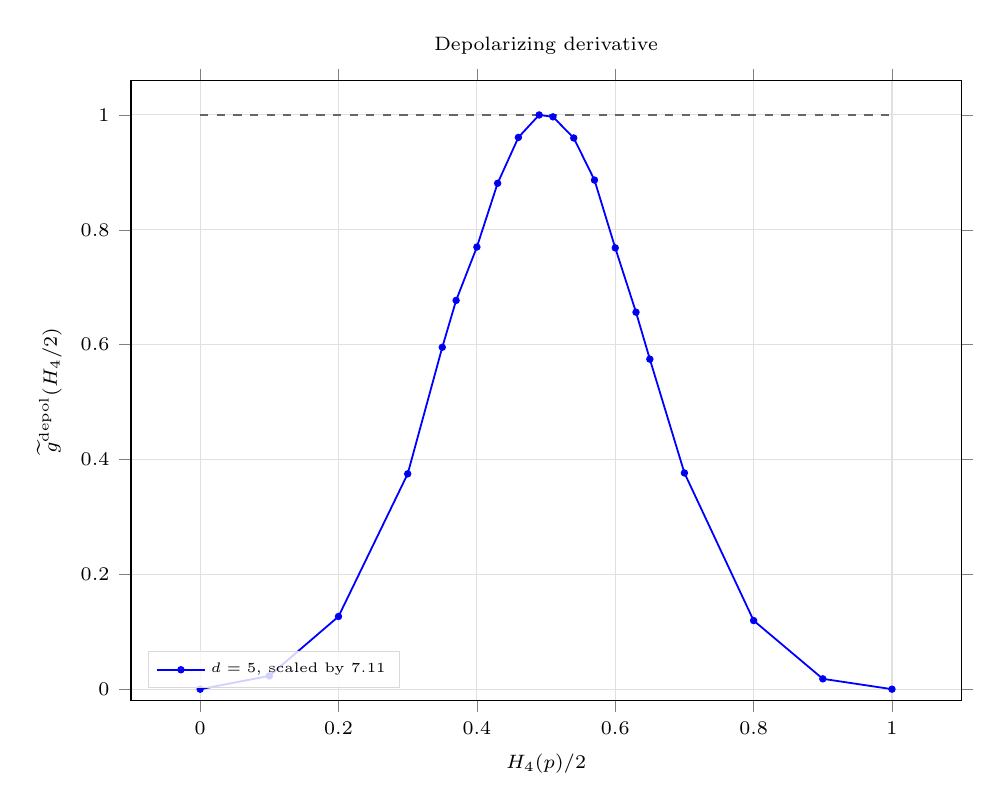
\begin{tikzpicture}
\begin{axis}[
  name=scaledDepolarizingGEXITSurface5Axis,
  width=\linewidth,
  height=0.78\linewidth,
  title={Depolarizing derivative},
  title style={font=\scriptsize},
  xlabel={$H_4(p)/2$},
  ylabel={$\widetilde g^{\rm depol}(H_4/2)$},
  ymin=-0.02, ymax=1.06,
  grid=both,
  major grid style={black!12},
  minor grid style={black!6},
  tick align=outside,
  tick label style={font=\scriptsize},
  label style={font=\scriptsize},
  legend cell align={left},
  legend style={draw=black!15, fill=white, fill opacity=0.82, text opacity=1, at={(0.02,0.02)}, anchor=south west, font=\tiny},
]
\addplot[black!60, dashed, line width=0.55pt, forget plot] coordinates {(0,1) (1,1)};
\addplot+[color=blue, mark=*, mark size=1.0pt, line width=0.65pt]
coordinates {(0,0) (0.1,0.0231252013791) (0.2,0.126603002342) (0.3,0.375012534461) (0.35,0.595409728769) (0.37,0.677070325975) (0.4,0.769998155027) (0.43,0.881000538857) (0.46,0.960872147817) (0.49,1) (0.51,0.996728698583) (0.54,0.959878469441) (0.57,0.886582284073) (0.6,0.76850463298) (0.63,0.656474564855) (0.65,0.574721364111) (0.7,0.376565494666) (0.8,0.119534693579) (0.9,0.0180571703987) (1,0)};
\addlegendentry{$d=5$, scaled by $7.11$}
\end{axis}
\end{tikzpicture}
